\documentclass{article}[article]

\usepackage{amsmath}
\usepackage{graphicx}
\usepackage{hyperref}

\graphicspath{ {./assets/} }

\title{Study Guide for Midterm One \\
        Chris Nutter \\
        Jared Dyreson}

\hypersetup{
    colorlinks,
    citecolor=black,
    filecolor=black,
    linkcolor=black,
    urlcolor=black
}

\begin{document}

\maketitle
\tableofcontents

\newpage

\section{Lectures}

%\begin{center}\fbox{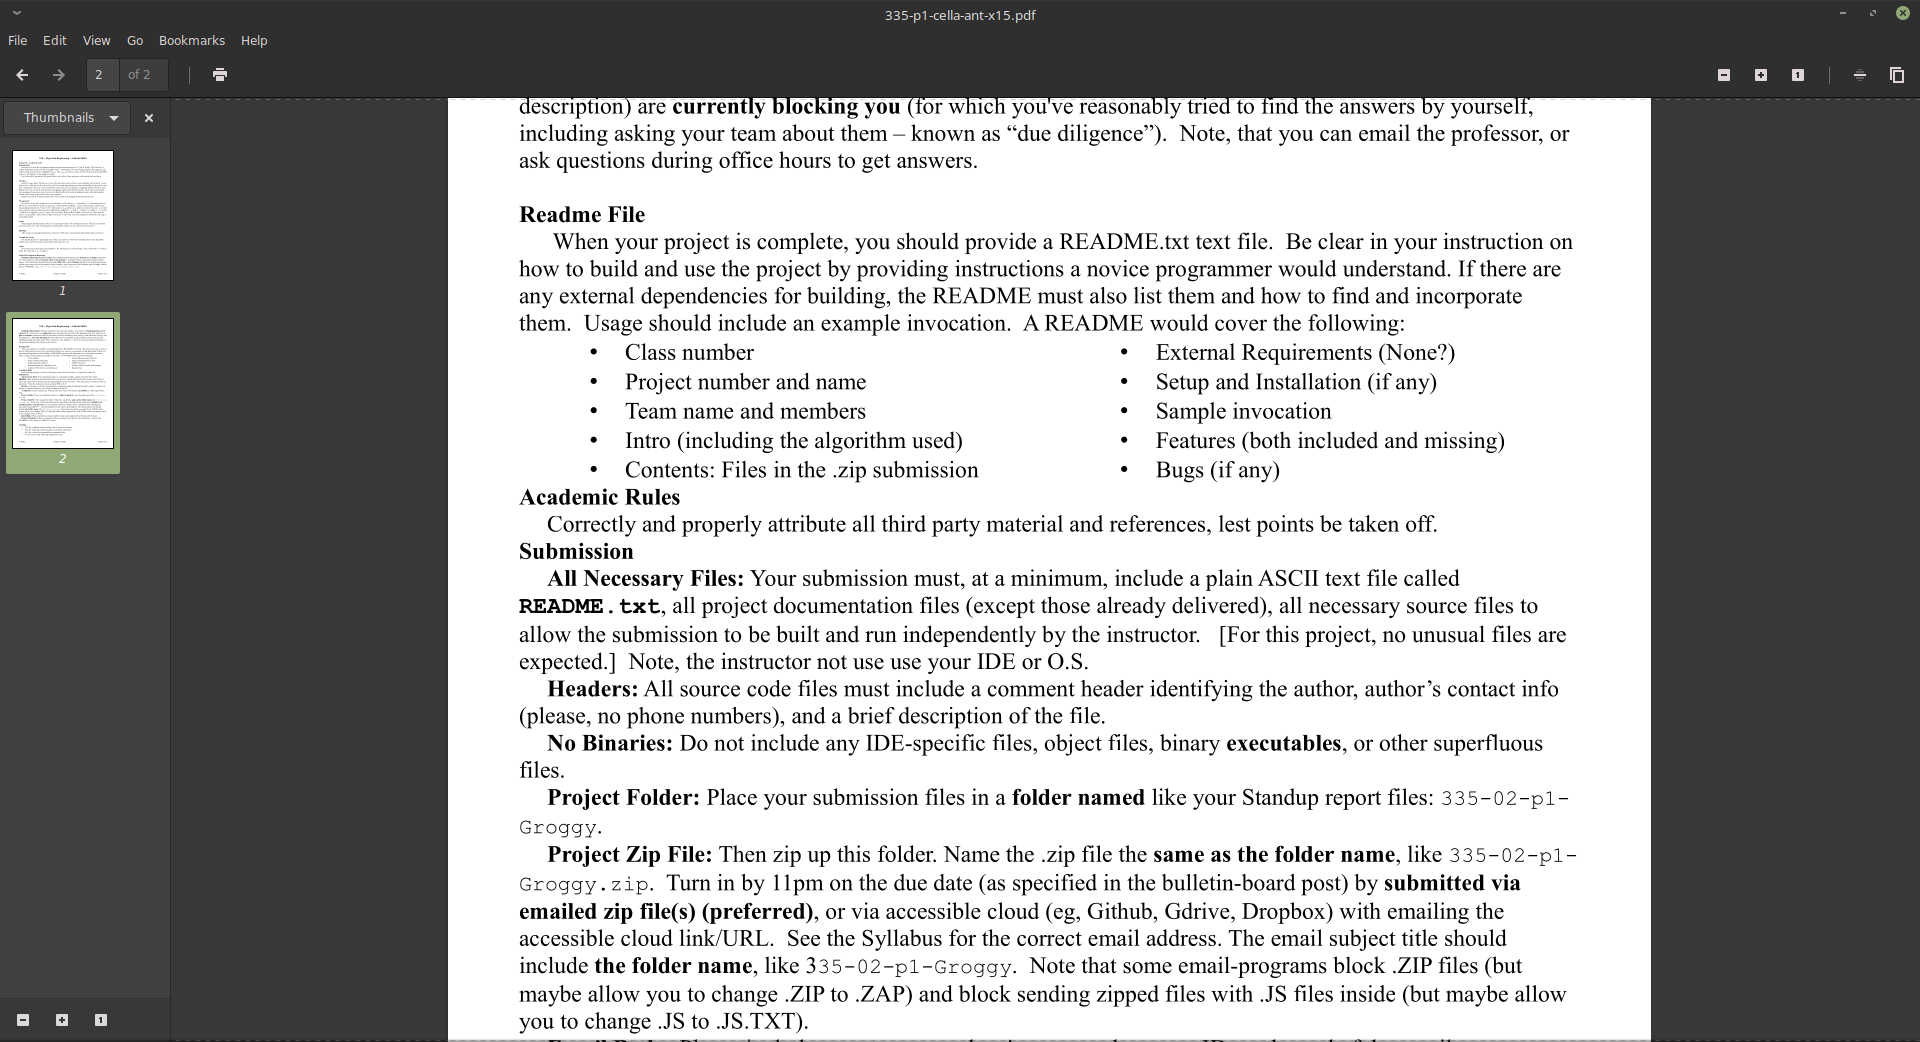
\includegraphics[width=13cm]{image.png}}\end{center}

\newpage

\section{Textbook Readings}

\vspace*{50px}

\subsection{Chapter 1}

\vspace*{25px}

\large{\textbf{Summary:}}

\newpage

\subsection{Chapter 2}

\vspace*{25px}

\large{\textbf{Summary:}}

Finite state machines can be thought of as black boxes that have a graphical representation.
Starting at a particular node, each input given can change the current state of the machine.
Changing state can be seen as moving along to another node, or simply looping on the current node, making no further progress.
We also have two distinctions for each node:

\begin{itemize}
\item Accepting state: desired position (there can be more than one)
\item Unaccepted state: undesired position
\end{itemize}

With FSMs, we can draw to different categories:

\begin{itemize}
\item NFA: Non-deterministic finite automa
\item DFA: Deterministic finite automa
\end{itemize}

Deterministic refers to the path taken in a state machine given a particular input.
Let say, for example you give the string \emph{w = cccaaa} to the following FSM:

\begin{center}\fbox{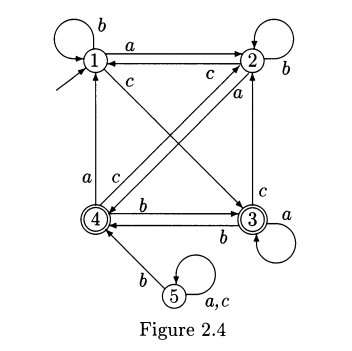
\includegraphics[width=13cm]{FSM.png}}\end{center}

The current path can be constructed:

\begin{center}\fbox{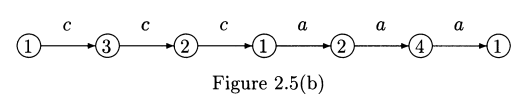
\includegraphics[width=13cm]{FSM_Path_M1.png}}\end{center}

\textbf{From my understanding, this mapping is a DFA. Meaning since we know the input we will know the given path taken by that input}

However, there are some machines where you don't know the path the machine can take.
These are NFAs and they have the state-transition function of:

$$N: Q \times (\Sigma \cup \{\epsilon\}) \rightarrow \mathcal{P}(Q)$$


\subsubsection{Subset Construction}

\href{https://www.youtube.com/watch?v=wYi3ThfLets}{Good video explanation}

\end{document}
